\documentclass[cjk,dvipdfmx,12pt,%
hyperref={bookmarks=true,bookmarksnumbered=true,bookmarksopen=false,%
colorlinks=false,%
pdftitle={第 42 回 関西 Debian 勉強会},%
pdfauthor={倉敷・のがた・佐々木},%
%pdfinstitute={関西 Debian 勉強会},%
pdfsubject={資料},%
}]{beamer}

\title{第 42 回 関西 Debian 勉強会}
\subtitle{{\scriptsize 資料}}
\author[佐々木 洋平]{{\large\bf 倉敷・のがた・佐々木}}
\institute[Debian JP]{{\normalsize\tt 関西 Debian 勉強会}}
\date{{\small 2010 年 12 月 26 日}}

%\usepackage{amsmath}
%\usepackage{amssymb}
\usepackage{graphicx}
\usepackage{moreverb}
\usepackage[varg]{txfonts}
\AtBeginDvi{\special{pdf:tounicode EUC-UCS2}}
\usetheme{Kyoto}
\def\museincludegraphics{%
  \begingroup
  \catcode`\|=0
  \catcode`\\=12
  \catcode`\#=12
  \includegraphics[width=0.9\textwidth]}
%\renewcommand{\familydefault}{\sfdefault}
%\renewcommand{\kanjifamilydefault}{\sfdefault}
\begin{document}
\settitleslide
\begin{frame}
\titlepage
\end{frame}
\setdefaultslide

\begin{frame}[fragile]
\frametitle{Agenda}

\tableofcontents

\end{frame}

\section{最近の Debian 関係のイベント}


\takahashi[40]{最近の Debian\\関係のイベント}
 

\begin{frame}[fragile]
\frametitle{第 41 回関西 Debian 勉強会 (1)}

\begin{itemize}
\item 日時: 11 月 6 日
\item 於: 関西オープンフォーラム (KOF) 2010
\end{itemize}

\begin{block}{ブース}
  物販, ネットブートによる Debian 体験
\end{block}
\begin{block}{セッション}
  Debian ランダムトピックス by 佐々木
\end{block}


\end{frame}
\begin{frame}[fragile]
\frametitle{第 41 回関西 Debian 勉強会 (2)       〜ブースの様子}

当日は Ubuntu Japanese Team の皆さんにもご協力頂きました

\begin{figure}[h]
    \centering
    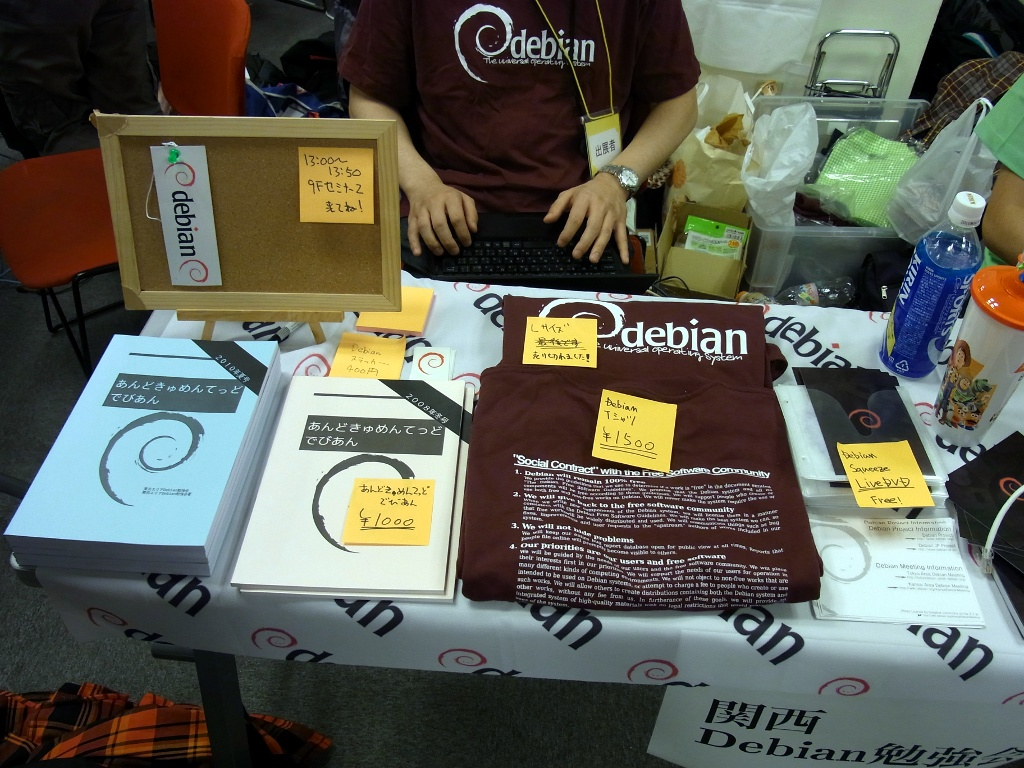
\includegraphics[width=0.45\textwidth]{image201012/kof1.jpg}
 \end{figure}


\end{frame}
\begin{frame}[fragile]
\frametitle{第 41 回関西 Debian 勉強会 (3)       〜セッションの様子}

野方さんの無茶振りで, 急遽矢吹さんによる御講演も.

\begin{figure}[h]
    \centering
    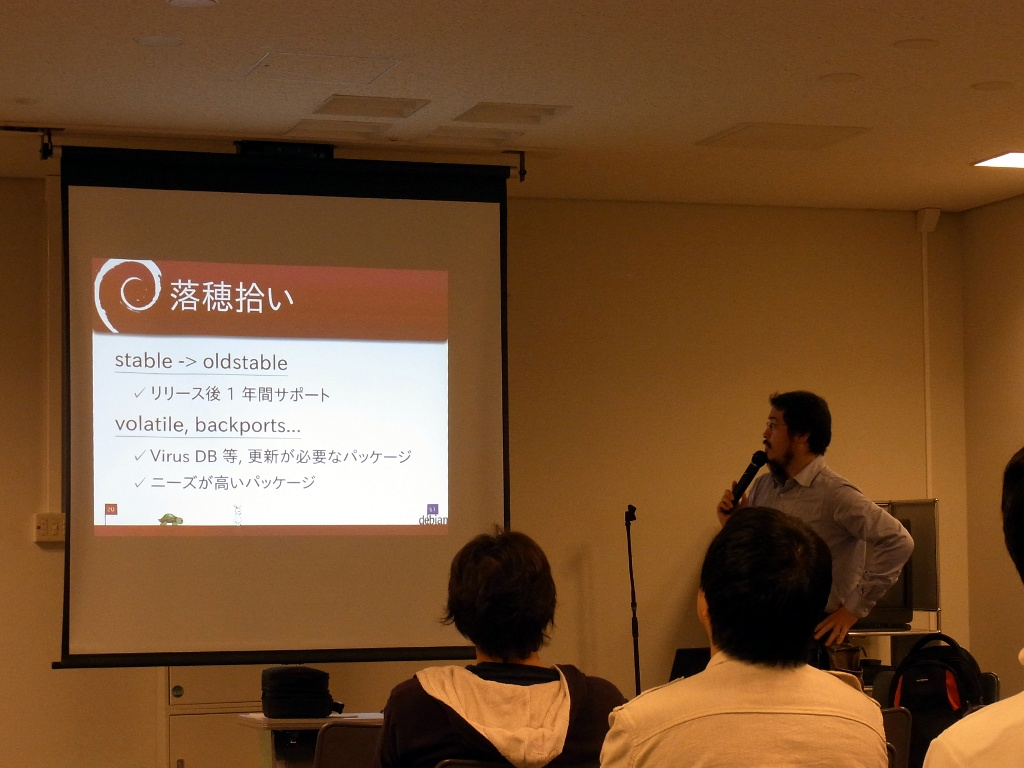
\includegraphics[width=0.45\textwidth]{image201012/kof2.jpg}
    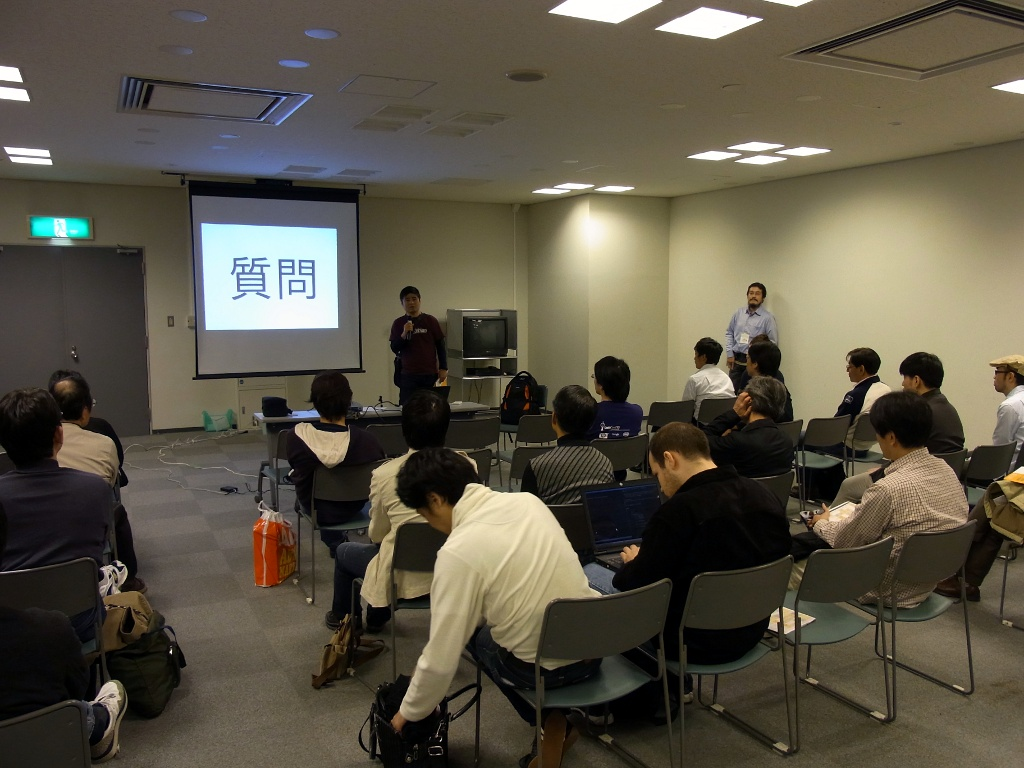
\includegraphics[width=0.45\textwidth]{image201012/kof4.jpg}
 \end{figure}


\end{frame}

\begin{frame}[fragile]
\frametitle{第 70 回東京エリア Debian 勉強会}

\begin{itemize}
\item 日時: 11 月 20 日
\end{itemize}

\begin{block}{テーマは「ファイルシステム」}
  \begin{itemize}
    \item Ext4, NILFS, BtrFS, CEPH...
    \item 最近のファイルシステムについて, これだけまとまった資料は無い, と思う. 興味のある方は御一読下さい
  \end{itemize}
{\scriptsize{\url{http://tokyodebian.alioth.debian.org/pdf/debianmeetingresume201011.pdf}}}
\end{block}

他に Debian Miniconf in Japan に関するブレスト等

\end{frame}


\section{事前課題発表}


\takahashi[50]{事前課題}


\begin{frame}[fragile]
\frametitle{今回の事前課題}


\begin{block}{「今年の反省と来年の計画」という目論見}
「 2011 年の関西 Debian 勉強会で発表する (されてほしい) トピックを 3 つ挙げてください
\end{block}


\end{frame}


\takahashi[50]{事前課題\\発表}


\begin{frame}[fragile]
\frametitle{川江}

\begin{itemize}
\item IPv6 について
\item HTML5 について
\item KVM について
\end{itemize}

\end{frame}

\begin{frame}[fragile]
\frametitle{ 上川純一 }

ひょっとすると参加かも

\end{frame}

\begin{frame}[fragile]
\frametitle{ 森山京平 }

\begin{itemize}
\item Vyatta について.
\item Debian でねっとわーく.
\item Linux プロセスマイグレーションを Debian で行う方法について.
\end{itemize}

\end{frame}

\begin{frame}[fragile]
\frametitle{ 甲斐正三 }

\begin{itemize}
\item Squeeze 上での日本語 TeX 環境構築

\begin{itemize}
\item できれば texworks で
\end{itemize}
\end{itemize}

\end{frame}

\begin{frame}[fragile]
\frametitle{ のがたじゅん }

\begin{itemize}
\item パッケージ作成は相変わらず需要が多いような気がします.
ほかは Web 関連と絡めて何か出来ればよいのかなと思ってます.
\item 自分でしゃべるネタとしては Debian Live は MultiArch や MultiFS, lxc などの機能
追加で相変わらず落ち着かないので, 新しいことを発表できるかと思います.
\end{itemize}

\end{frame}

\begin{frame}[fragile]
\frametitle{ かわだてつたろう }

\begin{itemize}
\item ドキュメント

\begin{itemize}
\item マニュアル, 翻訳, 査読などドキュメント全般にまつわること
\end{itemize}
\item ライセンス

\begin{itemize}
\item DFSG に適合するライセンス, しないライセンス
\item 適合するライセンスでもそれぞれの違い
\item 適合しないライセンスの問題点
\end{itemize}
\item リリースサイクル

\begin{itemize}
\item wheezy から固定リリースサイクルになってどのような変化があったのか
\end{itemize}
\end{itemize}

\end{frame}

\begin{frame}[fragile]
\frametitle{ dictoss (杉本  典充) }

\begin{itemize}
\item Debian のカーネル対決. (kLinux と kFreeBSD)
\end{itemize}

\end{frame}

\begin{frame}[fragile]
\frametitle{ 山田 洋平 }

\begin{itemize}
\item Debian パッケージの大分類「セクション」, または「 GNU R とは何か」
\item 組み込み開発のための Debian, Emdebian か何か
\item X11 のウィンドウマネジャですが何か.
\end{itemize}

\end{frame}

\begin{frame}[fragile]
\frametitle{ 山下康成 }

\begin{itemize}
\item apt V.S. aptitude
\item nano V.S. vim V.S. emacs etc.etc.
\item bash V.S. dash
\end{itemize}

全部, 宗教戦争?

\end{frame}

\begin{frame}[fragile]
\frametitle{ 佐々木洋平 }

\begin{itemize}
\item 4---6 月は開発者養成虎の穴, のようなルーチンワーク (ライセンスの確認, 基本的なパッケージ作成/ 管理)
\item OSC/KOF のセッションでは素人 (?) 向けと開発者 (含む予備軍) 向け, の二つやりませんか?
\item 他の勉強会とのクロスセッション. Emacs とか Gentoo とか\dots{}
\end{itemize}

と, リソース考えず言ってみるテスト.

\end{frame}

\begin{frame}[fragile]
\frametitle{ 木下 }

\begin{itemize}
\item 32bitOS から 64bitOS への移行関連
\item x86 系最新プラットフォームのサポート関連
\item Debian 最新バージョン情報関連
\end{itemize}

\end{frame}

\begin{frame}[fragile]
\frametitle{ lurdan }

\begin{itemize}
\item ゆるい分科会的なしかけを取り入れるのはどうかなぁ
\item 使いまわせる定番セッションの雛形資料を作って育てていくとか
\item 今年は一回しかできなかった puppet ネタをもう少しやりたいかも
\end{itemize}

\end{frame}

\begin{frame}[fragile]
\frametitle{ 松澤二郎 }

Debian 勉強会の雰囲気をよく把握できていないので的外れな回答になっているか
もしれませんが, 入門者向けのテーマを扱っていただけるとたいへん嬉しく思い
ます. 例えば,

\begin{itemize}
\item パッケージ作成講座や,
\item 今日からあなたも debian 翻訳者とか,
\item 渦巻きは何なのか
\end{itemize}

など, 初心者が知りたいことはたくさんあると思うので, そういうのは入り易く
て嬉しいですね. それで, 気がついたら Debian プロジェクトに巻き込まれてると.

\end{frame}


\takahashi[50]{そんな\\こんなで}
\takahashi[120]{次}



\section{Proxmox VE の紹介  by 森山京平 さん}


\takahashi[50]{Proxmox VEの紹介\\by\\森山京平さん}
\takahashi[50]{そんな\\こんなで}
\takahashi[120]{次}



\section{関西 Debian 勉強会 2010 年度各種イベント開催実績と総括}


\takahashi[20]{関西 Debian 勉強会 2010 年度各種イベント開催実績と総括}


\begin{frame}[fragile]
\frametitle{2010年の関西Debian勉強会}


 \begin{center}
  \begin{tabular}{|l|c|p{14em}|}
 \hline
 & 参加人数 & 内容 \\
 \hline
2010年1月 & 16 & Xen, 2010年企画 \\
2010年2月 & 16 & レンタルサーバでの利用, GAE \\
2010年3月 & 30? & OSC2010Kobe \\
2010年4月 & 12 & デスクトップ環境, 正規表現 \\
2010年5月 & 11 & ubuntu, squeeze \\
2010年6月 & 11 & debhelper7, cdbs, puppet \\
2010年7月 & 40? & OSC2010Kyoto \\
2010年8月 & 17 & emdebian, kFreeBSD \\
2010年9月 & 17 & タイルWM \\
2010年10月 & 12 & initramfs, debian live \\
2010年11月 & 33 & KOF2010 \\
2010年12月 & 14 & Proxmox, annual review \\
 \hline
  \end{tabular}
 \end{center}


\end{frame}

\begin{frame}[fragile]
\frametitle{出席者推移}


\begin{figure}[h]
 \begin{center}
  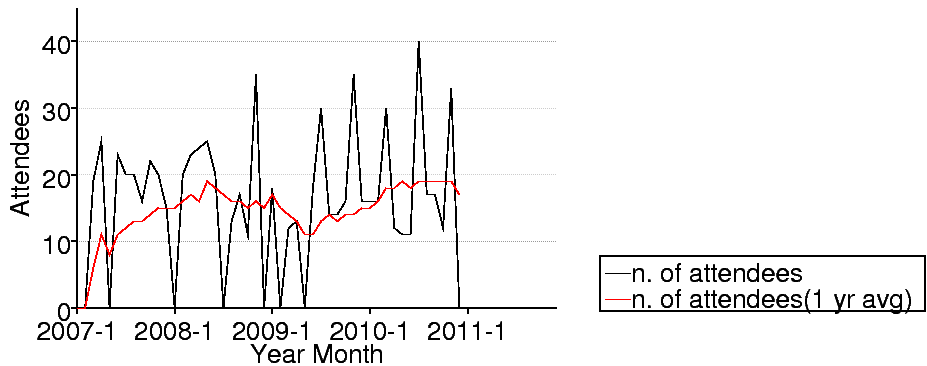
\includegraphics[width=1\hsize]{image201012/memberanalysis/kansai.png}
 \end{center}
\end{figure}


\end{frame}

\begin{frame}[fragile]
\frametitle{2010年の成果(?)}

\begin{itemize}
\item 東京の資料より
\end{itemize}

\begin{tabular}{lll}
  & 2009 年 & 2010 年 \\
\hline
DD になった人 & 矢吹, 谷口, 岩松 & やまねひでき \\
NM 中 & - & 岡部, 上野 \\
DM になった人 & - & 倉敷, 岡部, 佐々木 \\
Debian JP 加入 & - (佐々木?) & 1名(山田さん\@東京) \\
\end{tabular}

\end{frame}

\begin{frame}[fragile]
\frametitle{ネタを振り替える}

\begin{itemize}
\item 今年一月に所信表明演説をして頂きました.
\end{itemize}

\begin{tabular}{lll}
お名前 & 内容 & 発表 \\
\hline
杉本 & Debian GNU/kFreeBSD をホゲる & 8月発表 \\
甲斐 & 今年は Bug 報告頑張る & - \\
のがた & Debian Live をホゲる & 10月発表 \\
佐々木 & 野良を公式に upload & 11月発表 \\
川江 & 動画サーバを作る & - \\
倉敷 & サーバ運用まわりのインフラをホゲる & 6月発表 \\
山下 & TeraStation に Debian 入れてホゲる & - \\
\end{tabular}

\end{frame}


\takahashi[50]{来年のネタを考えてみる}
\takahashi[50]{そんな\\こんなで}


\begin{frame}[fragile]
\frametitle{今後の予定}


\begin{block}{第 43 回関西 Debian 勉強会}
\begin{itemize}
  \item 日時: 12 月 26 日
  \item 会場: 大阪: 港区区民センター, 楓の間
  \item 内容: 未定
  \begin{itemize}
    \item リリースに向けて? リリースされてる?
    \item 新年会?
  \end{itemize}
\end{itemize}
\end{block}


\end{frame}



\takahashi[50]{  }


\end{document}
%%% Local Variables: 
%%% mode: japanese-latex
%%% TeX-master: t
%%% End: 
